The \textbf{DetailEditor.tsx} component provides an interface for modifying selected seats, managing seat groups, categories, and configuring standing areas. It plays a huge role in SeatGen’s user interaction system by allowing users to efficiently modify stadium layouts in a structured and intuitive manner.

\textbf{Key Responsibilities:}
\begin{itemize}
    \item \textbf{Editing Individual Seats:} Users can update seat tooltips, positions, and categories.
    \item \textbf{Managing Seat Groups:} Enables users to create, merge, and delete groups of seats.
    \item \textbf{Standing Area Editing:} Supports renaming and capacity adjustments for standing areas.
    \item \textbf{Category Assignment:} Allows users to assign pricing tiers and colors to seats.
\end{itemize}

\subsection{Component Structure}
The \textbf{DetailEditor.tsx} has the following core sections:
\begin{itemize}
    \item \textbf{Seat Editing Panel:} Displays detailed information for selected seats and allows modifications.
    \item \textbf{Group Management Panel:} Handles seat grouping and bulk operations.
    \item \textbf{Standing Area Editing Panel:} Enables editing of standing areas, including name and capacity.
    \item \textbf{Deletion and Bulk Actions:} Supports removing selected seats, groups, or selected standing areas.
\end{itemize}

\begin{figure}[H]
    \centering
    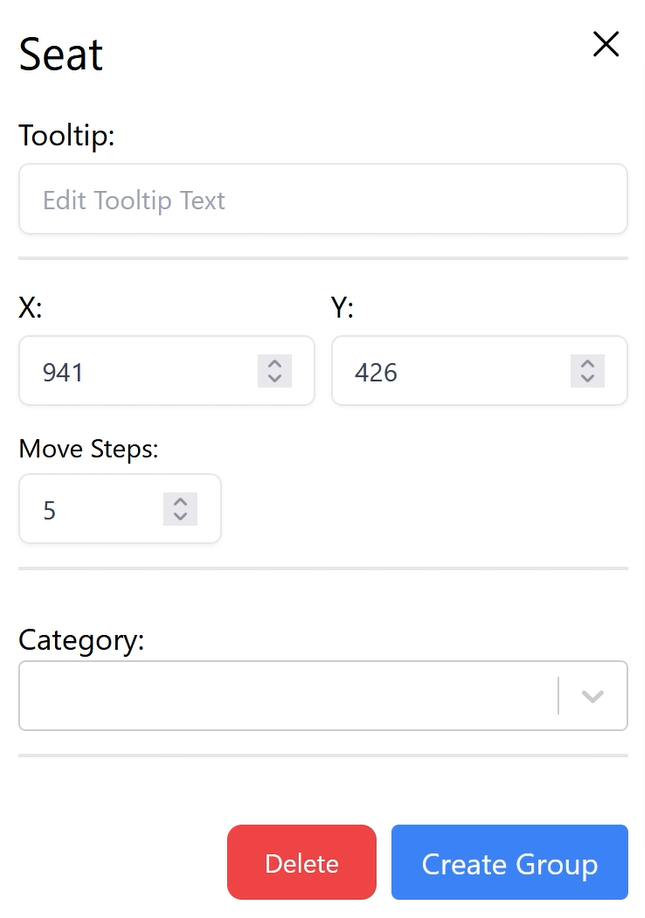
\includegraphics[width=0.6\textwidth]{pics/DetailEditorSeat.png}
    \caption{Seat Editing Panel in DetailEditor.tsx}
    \label{fig:detail-editor-seat}
\end{figure}

Figure~\ref{fig:detail-editor-seat} illustrates the seat editing panel, where users can adjust tooltips, assign categories, and delete seats.

\subsection{Managing Seat Attributes}
When a seat is selected, the editor provides multiple options for modification.

\subsubsection{Updating Tooltip Text}
Users can edit tooltip descriptions for seats, making it easier to add position information or other special notes.

\begin{lstlisting}[language=TypeScript, caption=Updating Tooltip for Selected Seats, label=lst:update-tooltip]
<input
    type="text"
    value={props.currentTooltip}
    onChange={props.handleExternalTooltipChange}
    placeholder="Edit Tooltip Text"
/>
\end{lstlisting}

\textbf{How It Works:}
\begin{itemize}
    \item The text input dynamically updates the tooltip for all selected seats by calling the \texttt{handleExternalTooltipChange} function.
    \item Changes are stored in the global state.
    \item Provides immediate visual feedback to the user.
\end{itemize}

\subsubsection{Adjusting Seat Position via UI}
Instead of manually dragging seats on the map, users can fine-tune their positions numerically. Also, adjusting the steps of one increment when using the arrow keys to position the seats perfectly is possible.

\begin{lstlisting}[language=TypeScript, caption=Updating Seat Coordinates, label=lst:update-seat-position]
const updateSeatPosition = (x: number, y: number) => {
    const latLng = props.mapRef.current!.layerPointToLatLng(new L.Point(x, y));
    props.updateSelectedSeatsPosition(selectedSeats[0].id, { lat: latLng.lat, lng: latLng.lng }, true);
};
\end{lstlisting}

\textbf{How It Works:}
\begin{itemize}
    \item Converts user-inputted X/Y values into map coordinates.
    \item Updates seat position dynamically.
    \item With this the movement is optimized for both manual entry and real-time adjustments.
\end{itemize}

\subsection{Group Management and Multi-Selection}
Grouping seats allows users to efficiently manage large stadium sections.
\subsubsection{Groups and Multi Selection and Deletion}

SeatGen supports the concept of seat groups, allowing users to efficiently manipulate multiple seats at once. Grouping seats enables bulk operations such as movement, category assignment, and section-wide modifications, making it particularly useful for managing large stadium layouts.

\textbf{Use Cases for Seat Groups:}
\begin{itemize}
    \item \textbf{Bulk Editing:} Modify multiple seat attributes simultaneously.
    \item \textbf{Efficient Repositioning:} Move multiple seats while maintaining relative positioning.
    \item \textbf{Category Assignment:} Assign pricing tiers and access restrictions to an entire section.
    \item \textbf{Simplified Deletion:} Remove entire seat groups without manually selecting each seat.
\end{itemize}

\textbf{Creating a Seat Group:}
\begin{lstlisting}[language=TypeScript, caption=Creating Seat Groups, label=lst:create-seat-group]
const createGroup = useCallback(() => {
    context.doAction(new CreateGroupAction(setSeatGroups, selectedSeats));
}, [selectedSeats, context]);
\end{lstlisting}

\textbf{How It Works:}
\begin{itemize}
    \item The function retrieves all currently selected seats.
    \item The CreateGroupAction is executed, registering the selected seats as a group.
    \item The group ID is assigned, and the group is stored in the global state.
\end{itemize}

\textbf{Deleting a Seat Group:}
\begin{lstlisting}[language=TypeScript, caption=Deleting Seat Groups, label=lst:delete-seat-group]
const deleteGroup = useCallback((groupId: number) => {
    context.doAction(new DeleteGroupAction(setSeatGroups, groupId));
}, [context]);
\end{lstlisting}

\textbf{Group Deletion Process:}
\begin{itemize}
    \item The DeleteGroupAction removes all seats within that group using the groupId.
    \item The global context state updates accordingly.
    \item The operation is reversible via the undo stack.
\end{itemize}

Furthermore, users can merge existing groups or split them dynamically, enabling flexible seat management. This allows for unlimited subgrouping, making the editor more intuitive and efficient.

\subsubsection{Seat Categories}
\setauthor{Michael Ruep}

Seat categories allow users to classify seating arrangements based on (pricing) tiers, accessibility, and special designations such as VIP areas or restricted sections. In SeatGen, every seat can be assigned a category that determines its visual representation and ticketing attributes.

\begin{figure}[H]
    \centering
    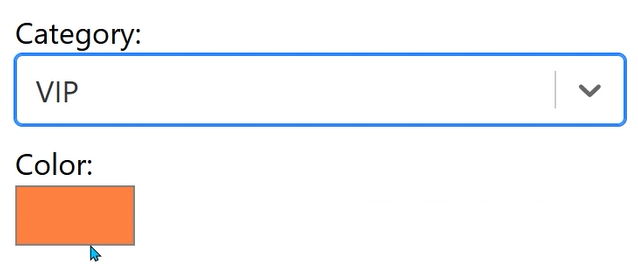
\includegraphics[width=0.7\textwidth]{pics/DetailEditorCategory.png}
    \caption{Category Selection in DetailEditor.tsx}
    \label{fig:detail-editor-category}
\end{figure}

\textbf{Features of Seat Categories:}
\begin{itemize}
    \item \textbf{Color-Coding:} Each category is assigned a color for clear visualization.
    \item \textbf{Pricing Information:} Categories define pricing tiers, ensuring correct ticket pricing.
    \item \textbf{Flexible Assignments:} Seats can be reassigned to different categories as needed.
    \item \textbf{Bulk Category Updates:} Multiple seats can be assigned a category simultaneously.
\end{itemize}

\subsubsection{Category Data Model}

Each seat category is stored as an object that holds classification data:

\begin{lstlisting}[language=TypeScript, caption=Seat Category Data Model, label=lst:seat-category-model]
interface Category {
    id?: number;
    name: string; // Example: "VIP", "General Admission"
    color: string; // Hex code for UI representation
    price: number; // Ticket price associated with this category
}
\end{lstlisting}

\subsubsection{Assigning Categories to Seats}

When a user selects a seat, they can assign or change its category using the \textbf{DetailEditor.tsx}.

\begin{lstlisting}[language=TypeScript, caption=Assigning Categories to Selected Seats, label=lst:assign-category]
const assignCategoryToSelectedSeats = (categoryId: number) => {
    context.setSeats(prevSeats => 
        prevSeats.map(seat => 
            seat.selected ? { ...seat, category: context.categories.find(c => c.id === categoryId) } : seat
        )
    );
};
\end{lstlisting}

\textbf{How It Works:}
\begin{itemize}
    \item The function loops through all selected seats.
    \item The new category is assigned based on the provided \texttt{categoryId}.
    \item The UI updates instantly, applying the new color and classification.
\end{itemize}

\subsubsection{Category Management in the UI}

Users can manage categories by:
\begin{itemize}
    \item Creating new categories with custom colors and pricing.
    \item Editing existing categories, updating names, prices, or colors.
    \item Deleting unused categories.
\end{itemize}

\begin{lstlisting}[language=TypeScript, caption=Managing Categories in Settings, label=lst:manage-categories]
const addCategory = (name: string, color: string, price: number) => {
    const newCategory: Category = { name, color, price };
    context.setCategories(prev => [...prev, newCategory]);
};
\end{lstlisting}

\subsubsection{Category Visualization on the Map}

Seat categories are visually represented by color-coded markers in \textbf{MapComponent.tsx}. Each seat marker dynamically updates based on its assigned category.

\begin{lstlisting}[language=TypeScript, caption=Rendering Seat Markers with Categories, label=lst:render-seat-category]
const renderedSeats = seats.map(seat => (
    <SeatMarker 
        key={seat.id} 
        seat={seat} 
        color={seat.category?.color || "gray"} 
        onClick={() => handleSeatClick(seat.id)}
    />
));
\end{lstlisting}

\textbf{How It Works:}
\begin{itemize}
    \item Each seat marker inherits the category's color.
    \item Unassigned seats default to a neutral color (gray).
    \item Selecting a seat allows users to change its category.
\end{itemize}

\subsubsection{Bulk Category Assignment Using Groups}

Seat groups enable bulk category assignments, allowing users to quickly change pricing tiers for multiple seats.

\begin{lstlisting}[language=TypeScript, caption=Assigning Categories to Seat Groups, label=lst:group-category-assignment]
const assignCategoryToGroup = (groupId: number, categoryId: number) => {
    setSeatGroups(prevGroups => 
        prevGroups.map(group => 
            group.id === groupId 
                ? { ...group, seats: group.seats.map(seat => ({ ...seat, category: context.categories.find(c => c.id === categoryId) })) }
                : group
        )
    );
};
\end{lstlisting}

\textbf{Advantages of Group Category Assignment:}
\begin{itemize}
    \item Speeds up pricing updates for entire sections.
    \item Reduces manual selection efforts.
    \item Ensures consistency in pricing and access restrictions.
\end{itemize}

\subsubsection{Conclusion}
Categories play a crucial role in SeatGen, providing a structured way to manage ticket pricing and seat classification. By integrating category assignment with group selection and bulk operations, users can efficiently update stadium layouts with minimal effort.

\subsection{Standing Area Editing}
\setauthor{Michael Ruep}
Standing areas in SeatGen are defined as polygonal sectors rather than individual seats. Unlike seats, which are represented as distinct markers, standing areas are implementd using a defined boundary of polygons. Each standing area has a name, and a maximum capacity.

\textbf{Key Features of Standing Areas:}
\begin{itemize}
    \item \textbf{Custom Polygonal Boundaries:} Users can define standing areas by selecting points on the map.
    \item \textbf{Capacity Control:} Each area has a maximum capacity limit.
    \item \textbf{Real-Time Editing:} Users can rename standing areas and adjust their capacities dynamically.
    \item \textbf{Deletion and Reconfiguration:} Existing standing areas can be removed or modified at any time.
\end{itemize}

\subsubsection{Standing Area Data Model}
Each standing area is stored as an object in the application state.

\begin{lstlisting}[language=TypeScript, caption=Standing Area Data Model, label=lst:standingarea-model]
interface StandingArea {
    id: number;
    name: string; // Display name of the standing area
    capacity: number; // Maximum allowed attendees
    coordinates: L.LatLng[]; // List of boundary points defining the area
    selected: boolean; // Boolean flag indicating selection state
}
\end{lstlisting}

\subsubsection{Creating and Selecting Standing Areas}
Standing areas are created by defining polygonal boundary coordinates on the map. Once an area is selected, it becomes editable in the \texttt{DetailEditor.tsx}.

\subsubsection{Renaming a Standing Area}
Users can rename standing areas directly in the \texttt{DetailEditor.tsx} panel.

\begin{lstlisting}[language=TypeScript, caption=Renaming Standing Areas, label=lst:rename-standingarea]
const handleStandingNameChange = (name: string) => {
    context.setStandingAreas(prev => prev.map(area =>
        context.selectedStandingAreaIds.includes(area.id)
            ? { ...area, name: name }
            : area
    ));
};
\end{lstlisting}

\textbf{How It Works:}
\begin{itemize}
    \item The function updates the name of all selected standing areas.
    \item Changes are reflected instantly in the UI.
    \item The new name is stored persistently for future sessions.
\end{itemize}

\subsubsection{Updating Standing Area Capacity}
To control attendee limits, each standing area has an adjustable capacity.

\begin{lstlisting}[language=TypeScript, caption=Updating Standing Area Capacity, label=lst:update-standingarea-capacity]
const handleStandingCapacityChange = (capacity: string) => {
    context.setStandingAreas(prev => prev.map(area =>
        context.selectedStandingAreaIds.includes(area.id)
            ? { ...area, capacity: Number(capacity) }
            : area
    ));
};
\end{lstlisting}

\textbf{Capacity Adjustment Process:}
\begin{itemize}
    \item The function modifies the capacity of all selected standing areas.
    \item Input validation ensures that only numeric values are accepted.
    \item The UI dynamically updates, reflecting the new ticketing constraints.
\end{itemize}

\subsubsection{Deleting a Standing Area}
Standing areas can be removed when no longer needed.

\begin{lstlisting}[language=TypeScript, caption=Deleting Standing Areas, label=lst:delete-standingarea]
const deleteSelectedStandingAreas = useCallback(() => {
    context.setStandingAreas(prev => prev.filter(area => 
        !context.selectedStandingAreaIds.includes(area.id)
    ));
    context.setSelectedStandingAreaIds([]);
}, [context]);
\end{lstlisting}

\textbf{How Deletion Works:}
\begin{itemize}
    \item The function filters out selected standing areas from the global state.
    \item The selection state resets to prevent unintended deletions.
    \item Deletion is undoable using the action history stack.
\end{itemize}

\begin{figure}[H]
    \centering
    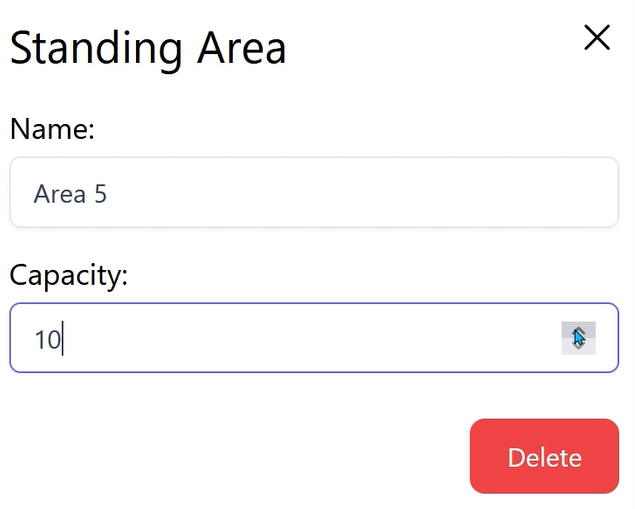
\includegraphics[width=0.7\textwidth]{pics/DetailEditorStandingArea.png}
    \caption{Editing Standing Areas in DetailEditor.tsx}
    \label{fig:detail-editor-standingarea}
\end{figure}

Figure~\ref{fig:detail-editor-standingarea} illustrates the interface for editing standing areas, including renaming, capacity adjustment, and deletion.

Standing areas in SeatGen offer a structured approach to handling non-seated sections of a stadium. By allowing dynamic capacity control and easy renaming, the system ensures that standing areas remain flexible and adaptable. Users can efficiently create, edit, and remove standing areas based on event needs, making stadium layouts highly customizable.

Beyond general standing areas, this feature can also be used to designate specific sections for specialized needs. For example, stadiums may allocate certain sectors for \textbf{wheelchair-accessible areas} or \textbf{priority seating for individuals with mobility impairments}. This flexibility ensures that accessibility requirements can be met while maintaining a clear and organized seating plan.

\subsubsection{Final Summary of DetailEditor.tsx}
\textbf{DetailEditor.tsx} is a key component within SeatGen, offering intuitive tools for modifying stadium layouts. It enables:
\begin{itemize}
    \item \textbf{Seat Editing:} Real-time adjustments to tooltips, positions, and assignments.
    \item \textbf{Group Management:} Merging, splitting, and deleting seat groups efficiently.
    \item \textbf{Category Assignment:} Bulk updates with intuitive color-coded visualization.
    \item \textbf{Standing Area Modifications:} Easy editing of boundaries and capacities.
    \item \textbf{Seamless Integration:} Ensures consistent updates via \texttt{MapContext.tsx}.
\end{itemize}

With its structured approach and live updates, \textbf{DetailEditor.tsx} ensures flexible and efficient stadium configuration.
